% --------------- PLANTILLA MAXI (GOD) -----------------
\documentclass[11pt, twocolumn]{article}

\usepackage[latin1,utf8]{inputenc}
\usepackage{verbatim}
\usepackage{multirow}
\usepackage{float}
\usepackage{enumerate}
\usepackage{graphics,graphicx,xcolor}
\usepackage{subfig}
\usepackage[spanish,es-tabla]{babel}
\usepackage{caption}
\usepackage{placeins}
\usepackage{afterpage}
\usepackage{blindtext}
\usepackage{multicol}
\usepackage{geometry}
\usepackage{lipsum}

%paquete para referencias
\usepackage[backend=biber, style=nature, citestyle=numeric, sorting=none, maxbibnames=99]{biblatex} % 
% \usepackage{natbib}
% \bibliographystyle{apsrev4-1} % Utiliza el archivo .bst de APS o uno similar

\usepackage{titling} % Paquete para personalizar título del documento
\usepackage{authblk}  % Paquete para personalizar autores del documento
\renewcommand\Authand{ y } % Reemplazar 'and' con 'y'

\DeclareCaptionFormat{custom}
{%
    \textbf{#1#2}\textit{\small #3}
}
\captionsetup{format=custom}

\newgeometry{bottom=3cm, top=2cm, left=3cm, right=3cm}
\usepackage{hyperref}
\hypersetup{
  colorlinks   = true, %Colours links instead of ugly boxes
  urlcolor     = blue, %Colour for external hyperlinks
  linkcolor    = black, %Colour of internal links
  citecolor   = black %Colour of citations
}

%paquete para unidades
\usepackage{siunitx}
% seteo punto como separador decimal
\AtBeginDocument{\decimalpoint}


% \DeclareSIUnit\torr{Torr}

%% Paquetes de la AMS
\usepackage{amsmath, amsthm, amsfonts, amssymb}

%componentes de texto
\usepackage{textcomp}


% Personaliza título del documento
\pretitle{\begin{center}\LARGE\bfseries}
    \posttitle{\par\vspace{0.5em}\end{center}\large}
    \preauthor{\begin{center}\large \lineskip 0.8em \begin{tabular}[t]{c}}
    \postauthor{\end{tabular}\par\end{center}}
    \predate{\begin{center}\large}
    \postdate{\par\end{center}}


\usepackage{fancyhdr}
\pagestyle{fancy}

% Definimos el encabezado de las paginas pares e impares.
\lhead{REDES NEURONALES}
\chead{Práctica 3 - 2024}
\rhead{Gatto Maximiliano}
\renewcommand{\headrulewidth}{0.5pt}

% aqui definimos el pie de pagina de las paginas pares e impares.
\lfoot[a1]{}
\cfoot[c1]{\thepage}
\rfoot[e1]{}

\renewcommand{\footrulewidth}{0.5pt}

% ------------------- TITULO ----------------------
% \title{\textbf{Procesamiento de imágenes digitales} \\ \vspace{1cm} \large IMÁGENES MÉDICAS - Práctica 2 - 2024}

\title{{\large REDES NEURONALES - PRÁCTICA 3 - 2024} \\ \vspace{1cm}\textbf{Estadística de trenes de spike}}



\author[ ]{\textbf{Maximiliano Gatto}}
\affil[ ]{Instituto Balseiro (UNCuyo - CNEA) - Bariloche, Río Negro, Argentina\vspace{0.4cm}}
\affil[ ]{\href{mailto:maximiliano.gatto@ib.edu.ar}{maximiliano.gatto@ib.edu.ar}}

\date{\today}

\begin{document}
\maketitle

% ------------------ INTRODUCCION ---------------------
\section{Introducción}
% En esta práctica se analiza la dinámica de sistemas acoplados correspondiente a neuronas. Especialmente el ejercicio 1 se implementó de manera numérica en un script de \texttt{Python}, cuyo código se encuentra disponible en el siguiente \href{https://github.com/elmasi2393/Redes-neuronales}{enlace}.

En esta práctica se analiza la estadística de trenes de spike mediante datos de estímulo y respuesta medidos experimentalmente por Ariel Rokem utilizando electrodos intracelulares en un saltamontes. Se proporcionaron 128 realizaciones de un estímulo sonoro durante \SI{1000}{\milli\second} dividido en ventanas de \SI{0.1}{\milli\second}, en donde se registró un 1 cuando se midió un spike y 0 en caso contrario. Los ejercicios se implementaron utilizando un script de \texttt{Python}, cuyo código se encuentra disponible en el siguiente \href{https://github.com/elmasi2393/Redes-neuronales/tree/main}{enlace}.


% ------------------ RESULTADOS ---------------------
\section{Resultados}

% --------------- INCISO 1 ---------------------
\subsection*{Ejercicio 1}
% En este inciso, se generó un histograma de los intervalos de los trenes de spike que se aproxime a la distribución de probabilidad \(P(\text{ISI})\) (\textit{inter-spike interval}) a partir de datos experimentales medidos con electrodos intracelulares en un saltamontes. En la Figura \ref{fig:estimulo_spikes} se puede observar el estímulo sonoro enviado al saltamontes, junto con los spikes medidos por los electrodos en un intervalo de \SI{1}{\milli\second}

Se generó un histograma de los intervalos entre spikes que aproxima la distribución \(P(\text{ISI})\), basado en datos medidos con electrodos intracelulares en un saltamontes. La Figura \ref{fig:estimulo_spikes} muestra el estímulo sonoro y los spikes registrados en intervalos de \SI{0.1}{\milli\second}.


\begin{figure} [htbp]
    \centering
    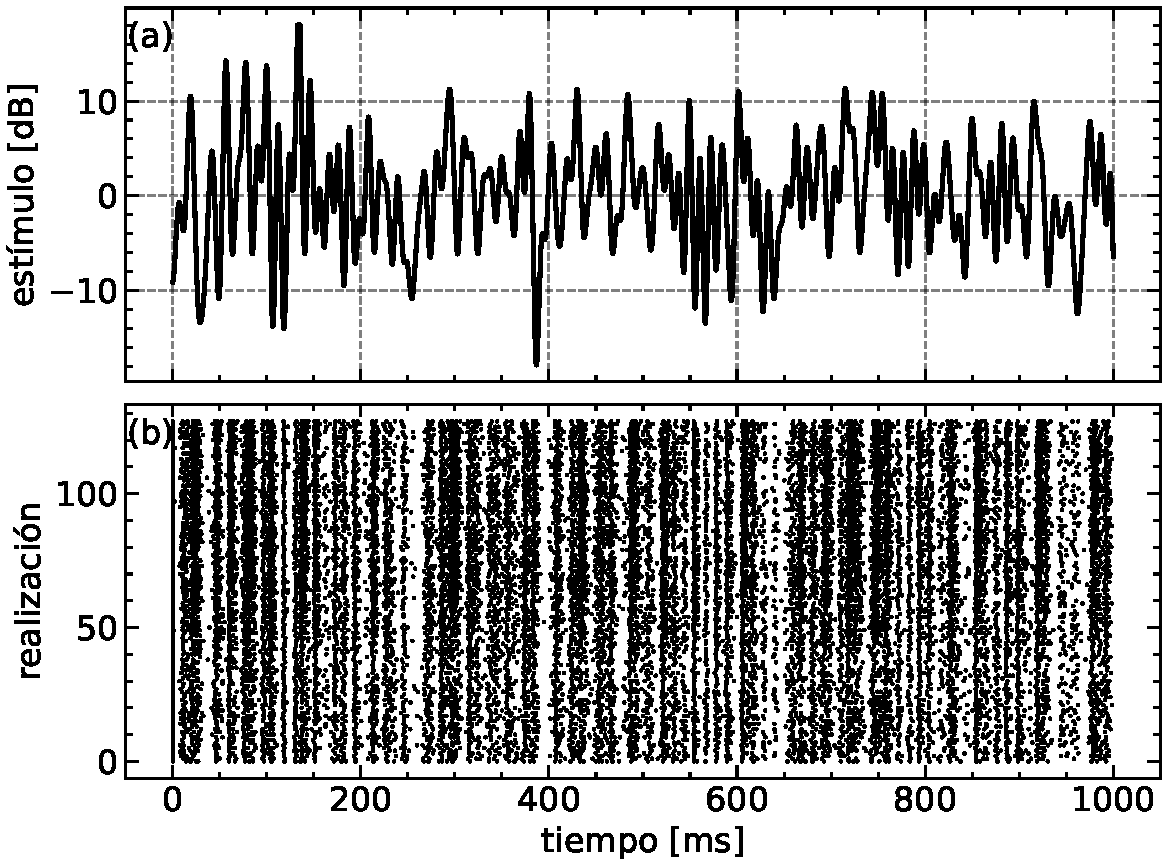
\includegraphics[width=0.45\textwidth]{figures/estimu_spikes.pdf}
    \caption{(a) estímulo sonoro enviado al saltamontes y (b) spikes medidos por los electrodos en un intervalo de \SI{1}{\milli\second} para cada realización.}
    \label{fig:estimulo_spikes}
\end{figure}


Para calcular el histograma de los intervalos de los trenes de spike, se consideraron todas las realizaciones del experimento. El resultado obtenido, se muestra en la Figura \ref{fig:histogram_ISI}.

\begin{figure} [htbp]
    \centering
    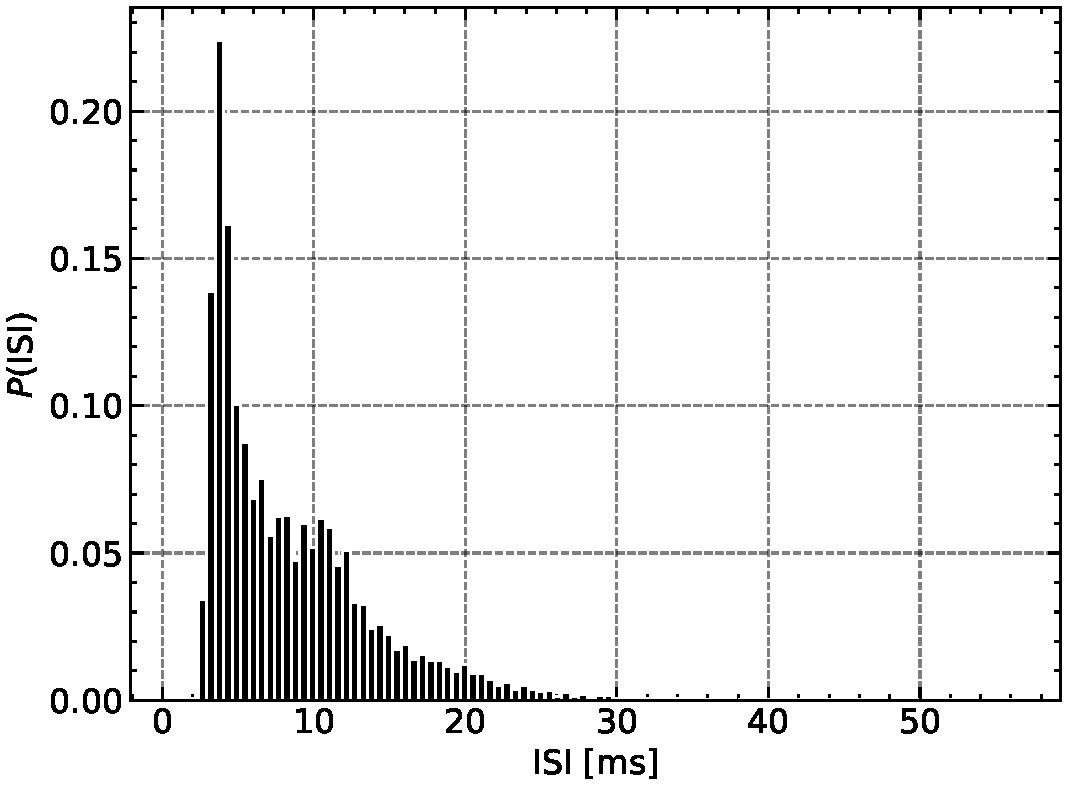
\includegraphics[width=0.45\textwidth]{figures/ISI.pdf}
    \caption{histograma de los intervalos de los trenes de spike ISI.}
    \label{fig:histogram_ISI}
\end{figure}

% Además, se calculo el coeficiente de variabilidad, definido como \(CV = \frac{\sigma_\text{ISI}}{\langle \text{ISI} \rangle}\), donde \(\sigma_\text{ISI}\) es la desviación estándar y \(\langle \text{ISI} \rangle\) es el valor medio de los intervalos de los trenes de spike. Se obtuvo un valor de \(CV = 0.6573\).

Se calculó el coeficiente de variabilidad, definido como \(CV = \frac{\sigma_\text{ISI}}{\langle \text{ISI} \rangle}\), obteniéndose \(CV = 0.6573\).

\subsection*{Ejercicio 2}
Se obtuvo un histograma que aproxima la probabilidad de obtener N spikes en una realización. Para ello, en cada una de las 128 realizaciones se contaron los spikes y se generó el histograma que se muestra en la Figura \ref{fig:histogram_Nspikes}.

\begin{figure} [htbp]
    \centering
    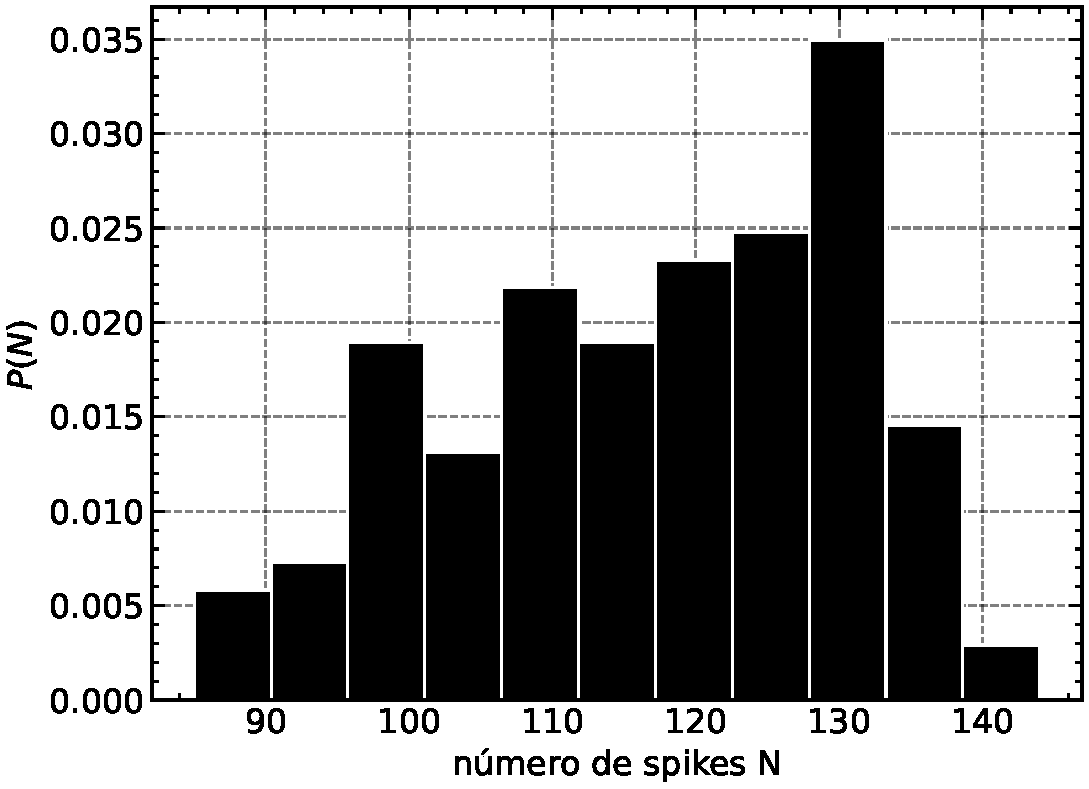
\includegraphics[width=0.42\textwidth]{figures/spikes_count.pdf}
    \caption{histograma de la cantidad de spikes en una realización.}
    \label{fig:histogram_Nspikes}
\end{figure}

% Luego, el factor de Fano se puede calcular como \(F = \frac{\sigma^2_N}{\langle N \rangle}\), donde \(\sigma^2_N\) es la varianza y \(\langle N \rangle\) es el valor medio de la cantidad de spikes en una realización. Se obtuvo un valor de \(F = 1.5657\), mientras que \(CV^2 = 0.4319\). Dado que \(F \neq CV^2\), se concluye que el proceso no es de tipo \textit{renewal}.

Luego, el factor de Fano se calculó como \(F = \frac{\sigma^2_N}{\langle N \rangle}\), obteniendo \(F = 1.5657\) y \(CV^2 = 0.4319\). Dado que \(F \neq CV^2\), el proceso no es de tipo \textit{renewal}.

\subsection*{Ejercicio 3}
Se estimó la tasa de disparo dependiente del tiempo \(r(t)\) de los datos experimentales promediando en todas las realizaciones utilizando un tamaño de ventana de 100 valores, que se corresponde con \SI{10}{\milli\second}. Es decir, cada realización se las dividió en ventanas de 100 valores, se promedió la cantidad de spikes en cada ventana y de dividió por el tamaño temporal de la ventana para obtener la tasa de disparo. El resultado obtenido se muestra en la Figura \ref{fig:rate}.

% Se estimó la tasa de disparo \(r(t)\) promediando los datos experimentales en ventanas de 100 valores (\SI{10}{\milli\second}). Cada realización, se dividió en ventanas donde se calculó el promedio de spikes y se dividió por el tamaño temporal. El resultado se muestra en la Figura \ref{fig:rate}.

\begin{figure} [htbp]
    \centering
    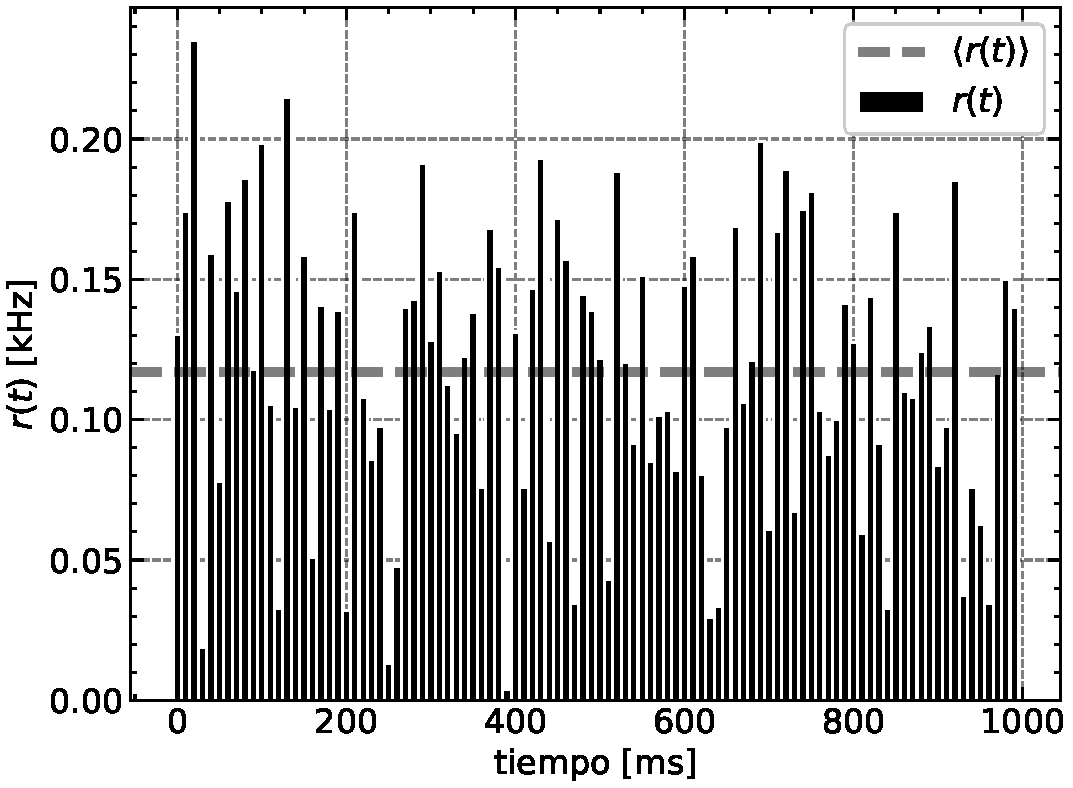
\includegraphics[width=0.45\textwidth]{figures/rate.pdf}
    \caption{tasa de disparo dependiente del tiempo \(r(t)\) de los datos experimentales.}
    \label{fig:rate}
\end{figure}

\subsection*{Ejercicio 4}
% Para calcular la mejor función filtro que da la mejor predicción lineal del histograma dependiente del tiempo \(r(t)\), despreciando el tiempo de autocorrelación del estímulo, se utilizó solo el filtro lienal \(D(\tau)\) suponiendo que el estímulo es ruido blanco. La función filtro se calcula como \(D(\tau) = \frac{C(\tau)}{\sigma^2_s}\), donde \(\sigma^2_s\) es la varianza del estímulo y \(C(\tau)\) está definido como

Para calcular el mejor filtro lineal para predecir \(r(t)\) despreciando el tiempo de autocorrelación del estímulo, se usó solo el filtro \(D(\tau)\), asumiendo que el estímulo es ruido blanco. El filtro se calcula como \(D(\tau) = \frac{C(\tau)}{\sigma^2_s}\), donde \(\sigma^2_s\) es la varianza del estímulo y \(C(\tau)\) es


\begin{equation}    \nonumber
    C(\tau) = \frac{1}{T N_\text{trials}} \sum_\text{spikes} S(t_\text{spike} - \tau),
\end{equation}

\noindent donde \(S(t)\) es el estímulo,\(N_\text{trials}\) es la cantidad de realizaciones y \(T\) es el tiempo total de la realización. El resultado obtenido se muestra en la Figura \ref{fig:filter}.

\begin{figure} [htbp]
    \centering
    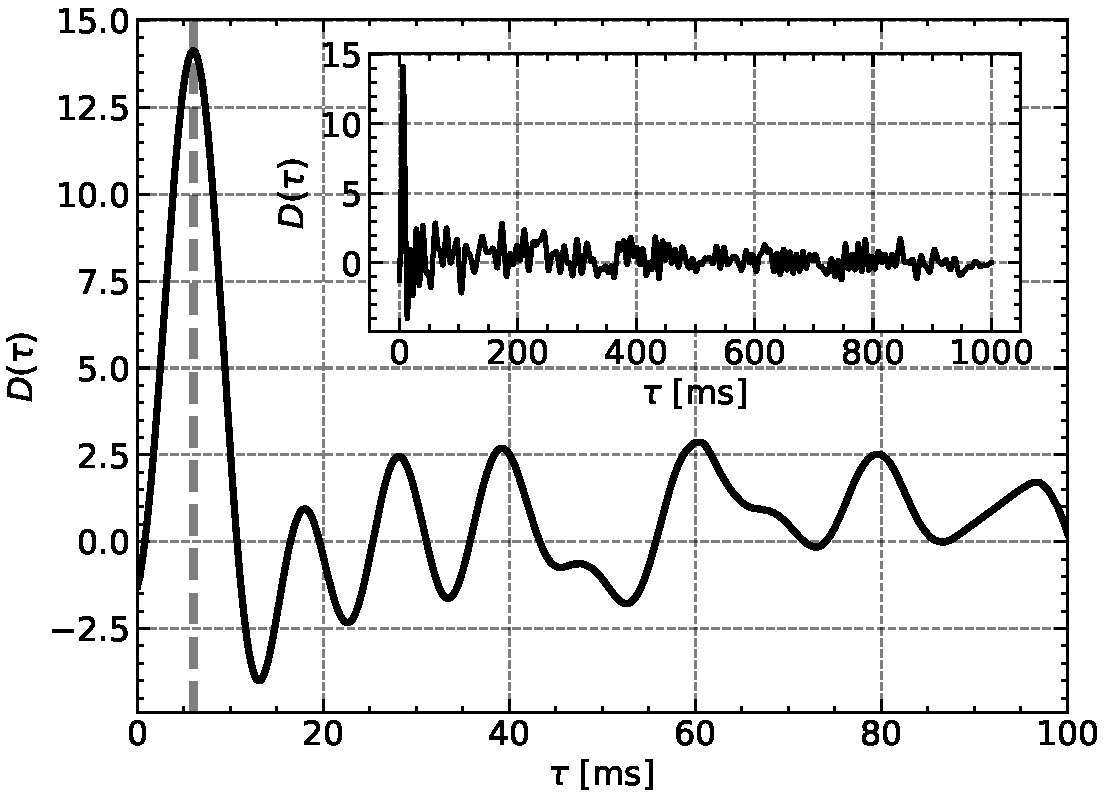
\includegraphics[width=0.45\textwidth]{figures/correlogram.pdf}
    \caption{función filtro \(D(\tau)\) que da la mejor predicción lineal del histograma dependiente del tiempo \(r(t)\).}
    \label{fig:filter}
\end{figure}

En la Figura \ref{fig:filter} se puede ver que la función filtro \(D(\tau)\) es máxima cuando \(\tau =\) \SI{6}{\milli\second}, lo que indica que la correlación entre el estímulo y la tasa de disparo es máxima en ese tiempo, es decir la neurona responde al estímulo con un retardo de \SI{6}{\milli\second}.

\end{document}